\documentclass{paper}
\usepackage{gary}
\usepackage{subfigure}
\usepackage[margin=1in]{geometry}
\usepackage{mwe}
\title{Modeling Frequency of Terrorist Attacks}
\author{Gary Cheng and Preetham Gujjula}

\begin{document}
\maketitle 

\section{Introduction}

\begin{figure}
\centering
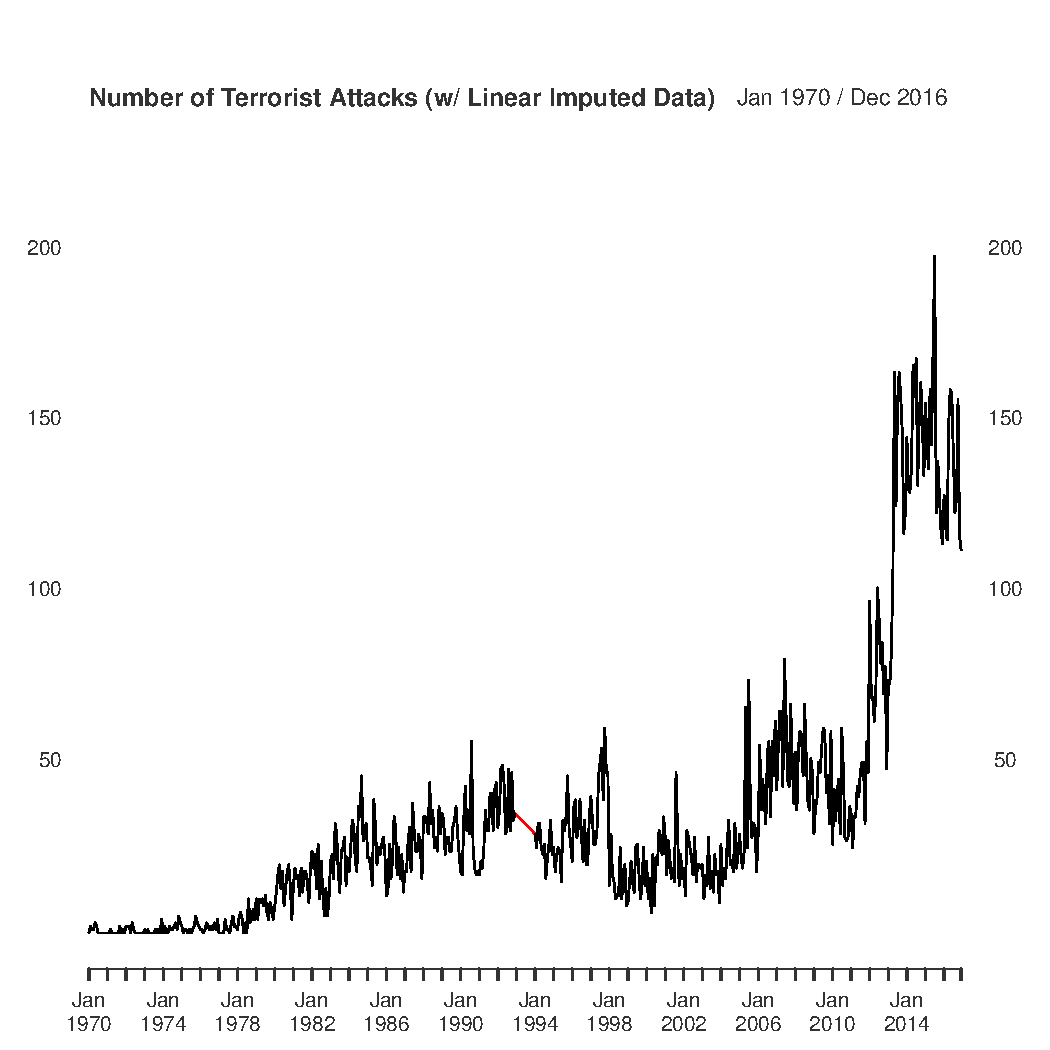
\includegraphics[width=0.75\linewidth]{../image/og_ts.pdf}
\caption{The original time series with a linear imputation (in red) for the missing data in 1993.}
\label{og}
\end{figure}

\begin{figure}
\centering
    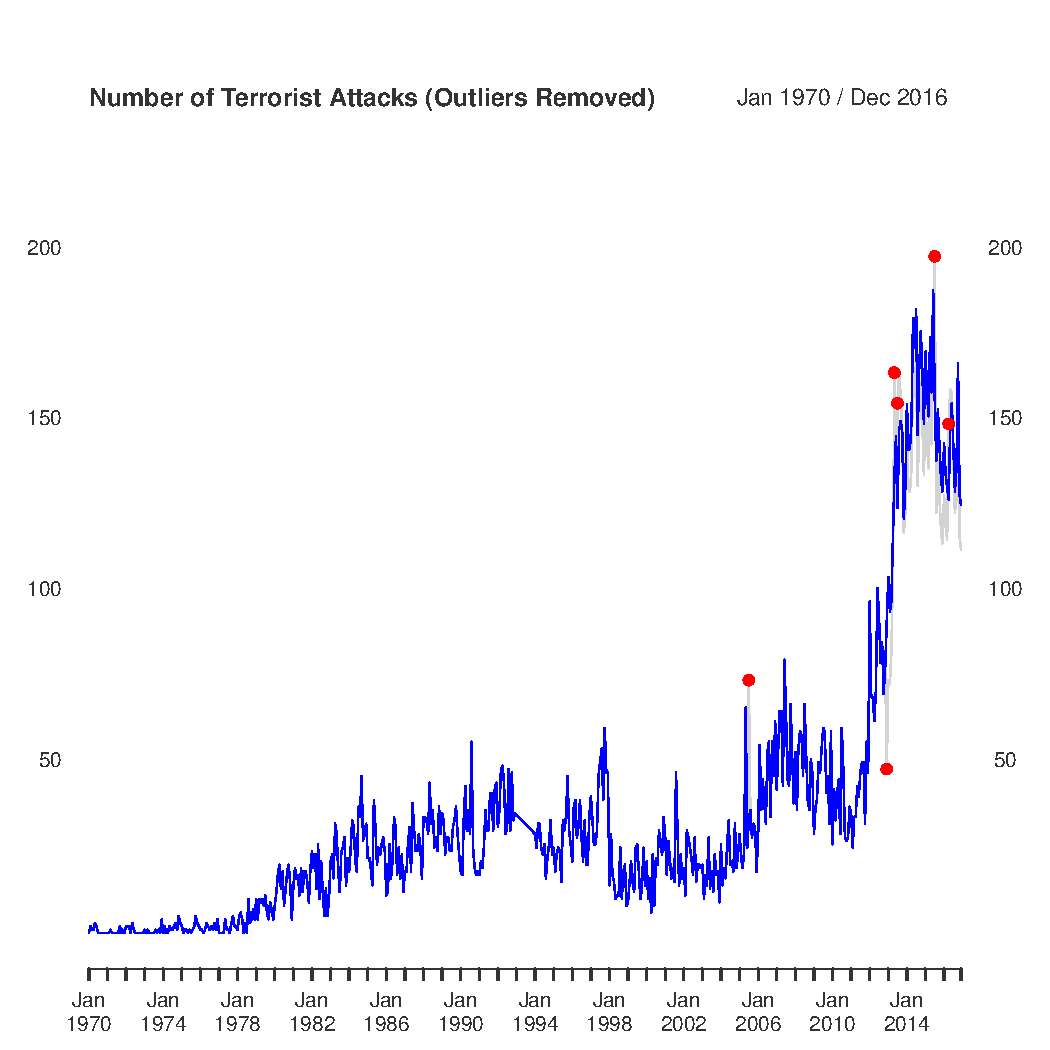
\includegraphics[width=0.75\textwidth]{../image/outlier_comparison.pdf}
\caption{The imputed time series (in blue) with outliers removed. The original time series shown in gray. The 6 outliers are shown in red. }
\label{outlier}
\end{figure}

\begin{figure}
\centering
    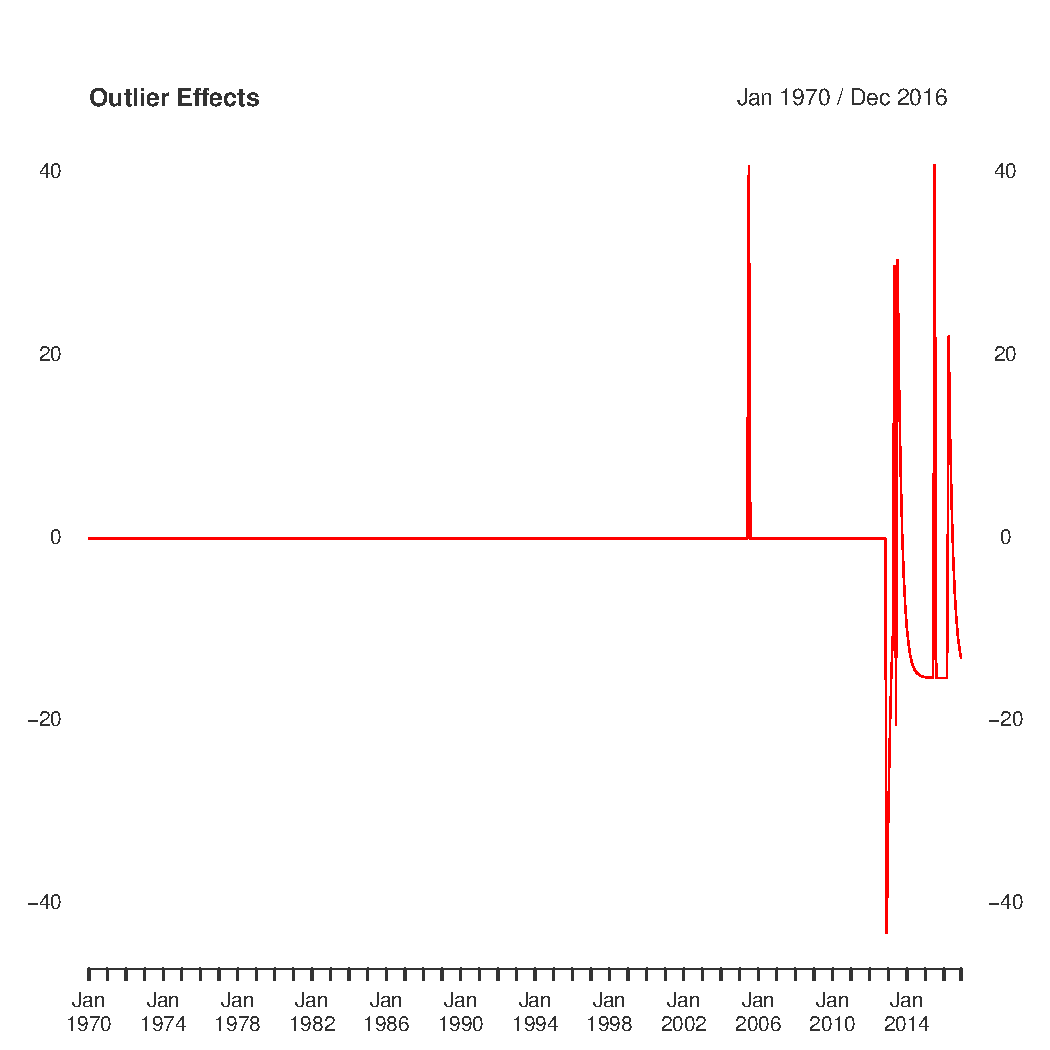
\includegraphics[width=0.75\textwidth]{../image/outlier_effects.pdf}
\caption{The outlier effects of the identitifed outliers are displayed here.}
\label{outlier}
\end{figure}



\begin{figure}
\centering
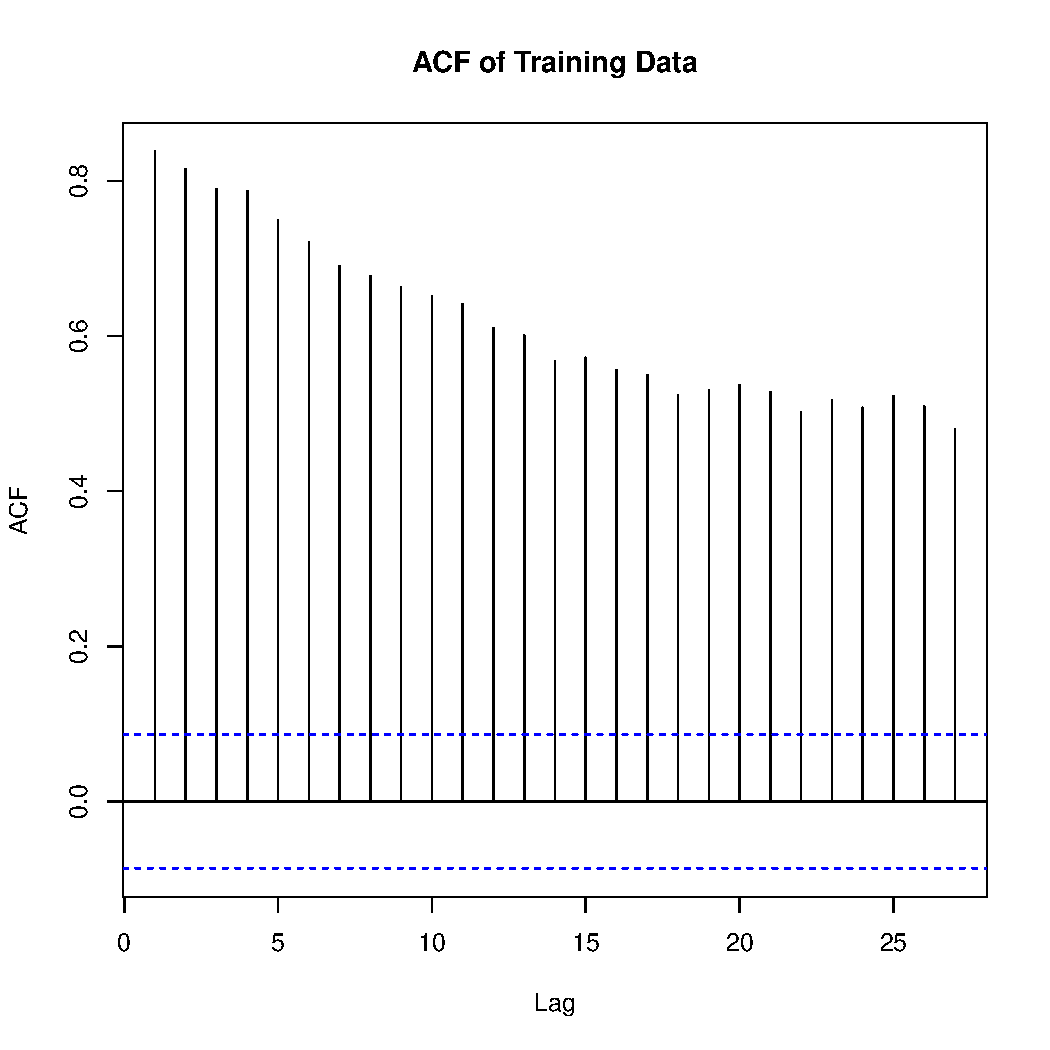
\includegraphics[width=0.45\linewidth]{../image/acf_og.pdf}
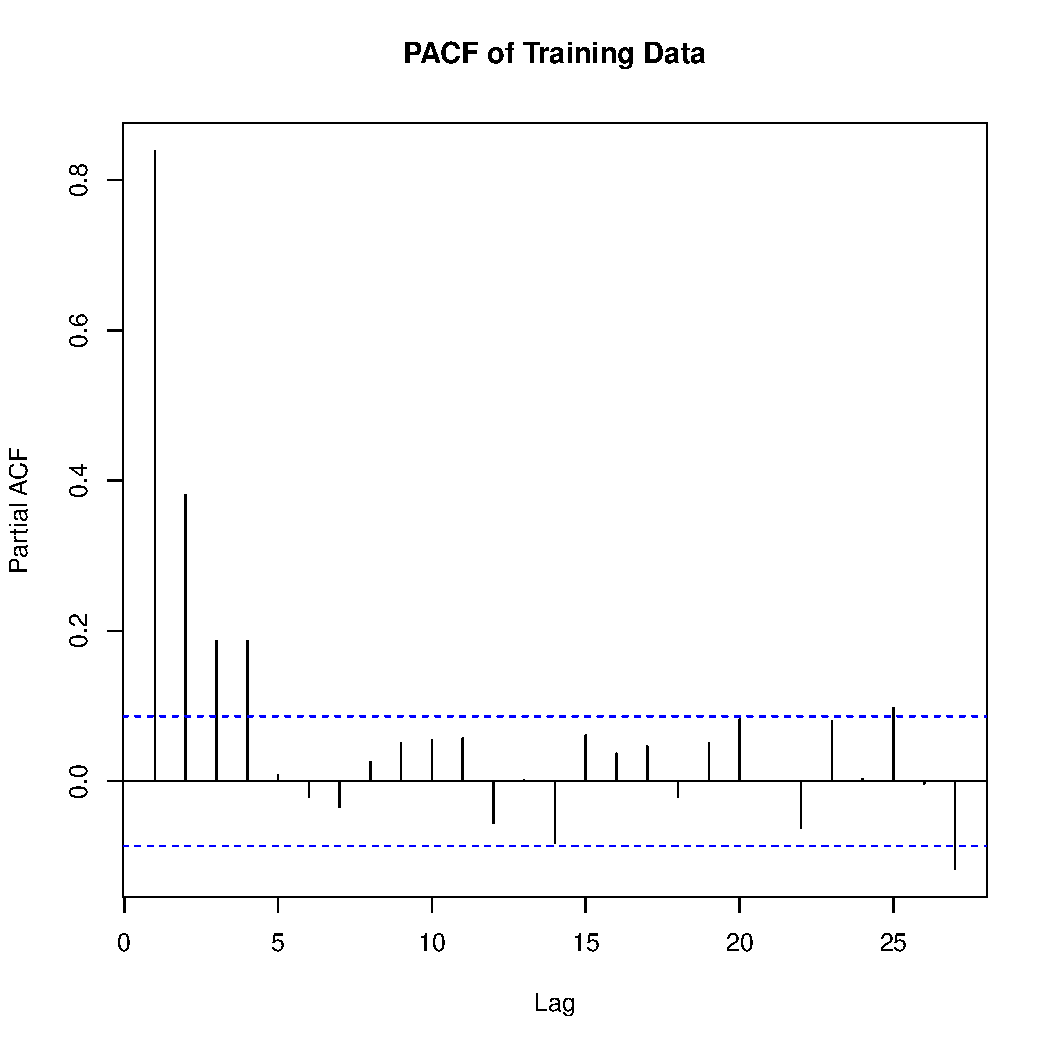
\includegraphics[width=0.45\linewidth]{../image/pacf_og.pdf}
\caption{The ACF and PACF of the time series}
\label{og_acf_pacf}
\end{figure}



\begin{figure}
\centering
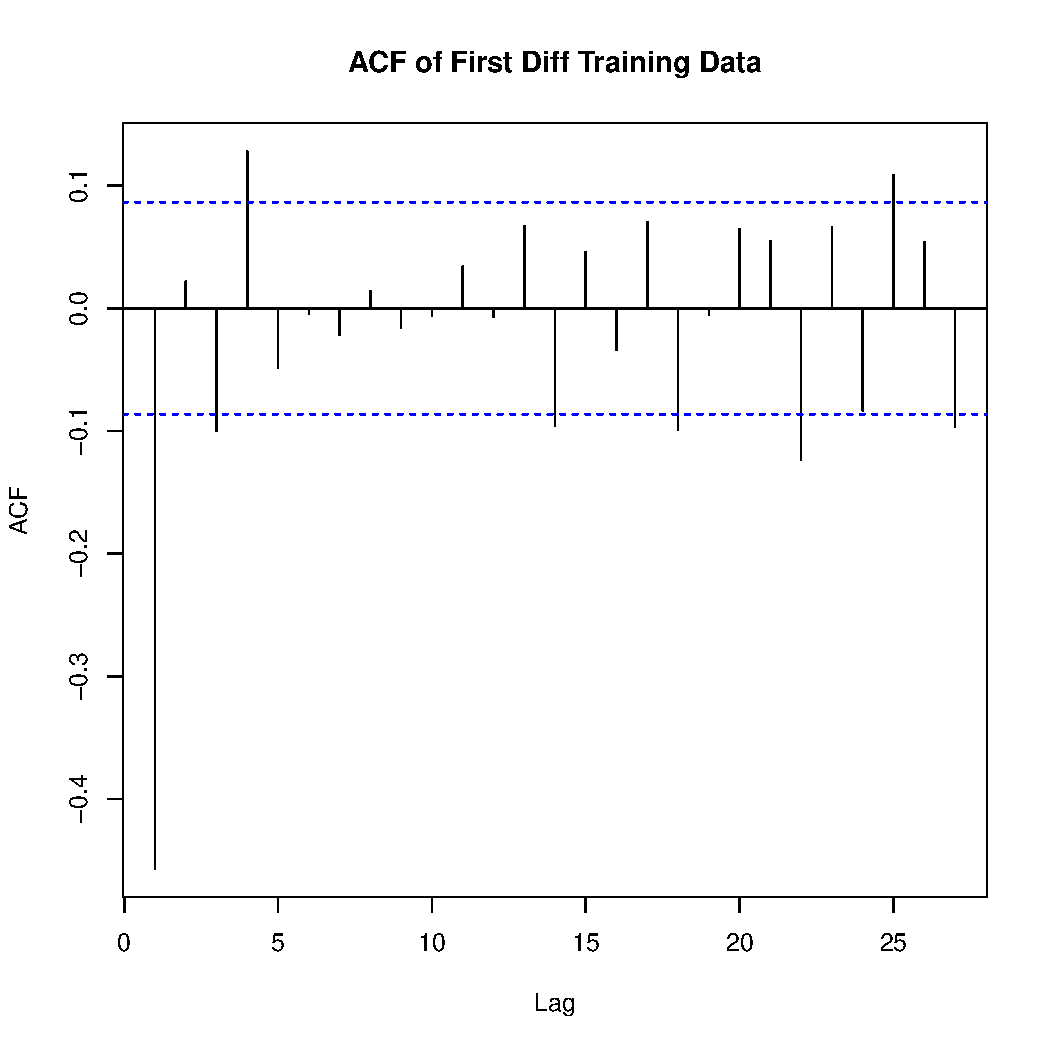
\includegraphics[width=0.45\linewidth]{../image/acf_first_diff.pdf}
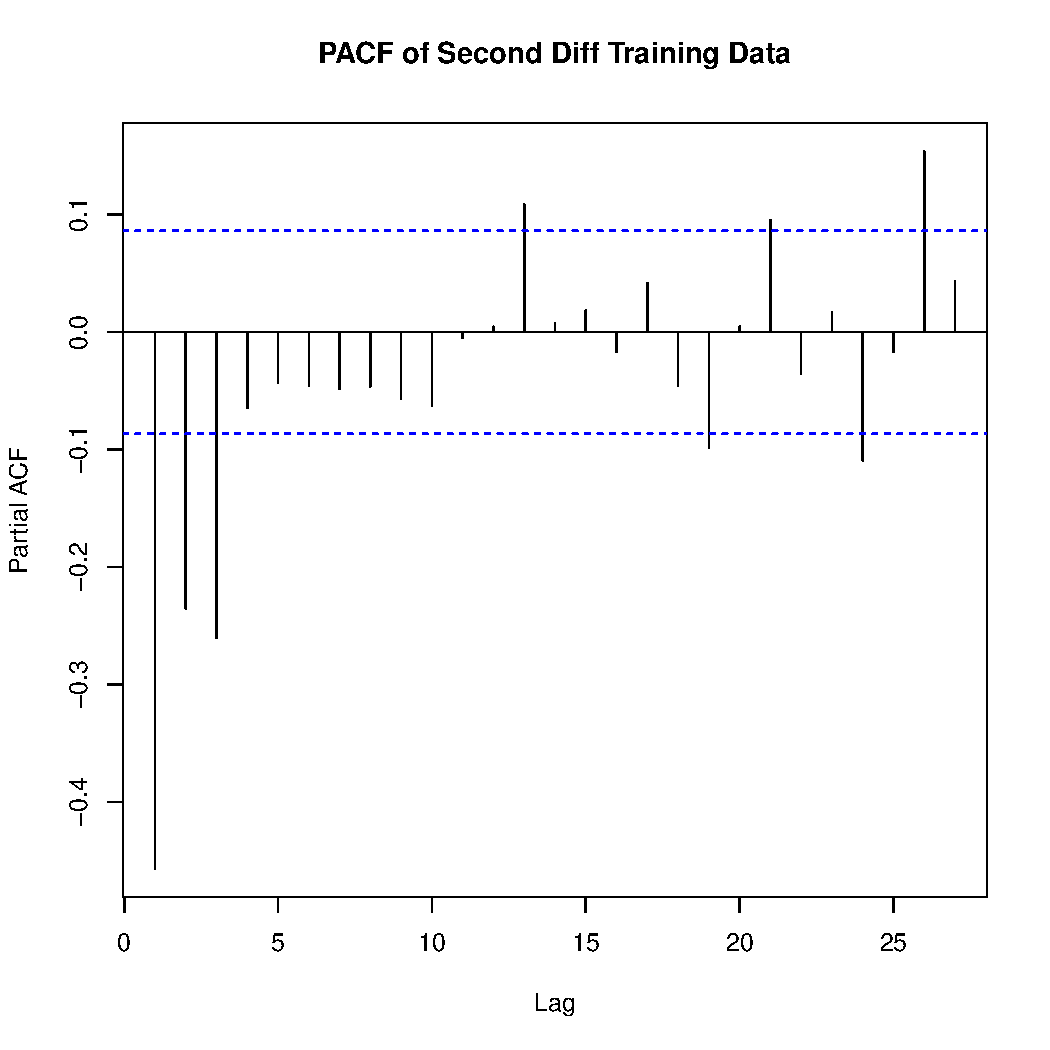
\includegraphics[width=0.45\linewidth]{../image/pacf_second_diff.pdf}
\caption{The ACF and PACF of the first diff time series}
\label{first_acf_pacf}
\end{figure}

\begin{figure}
\centering
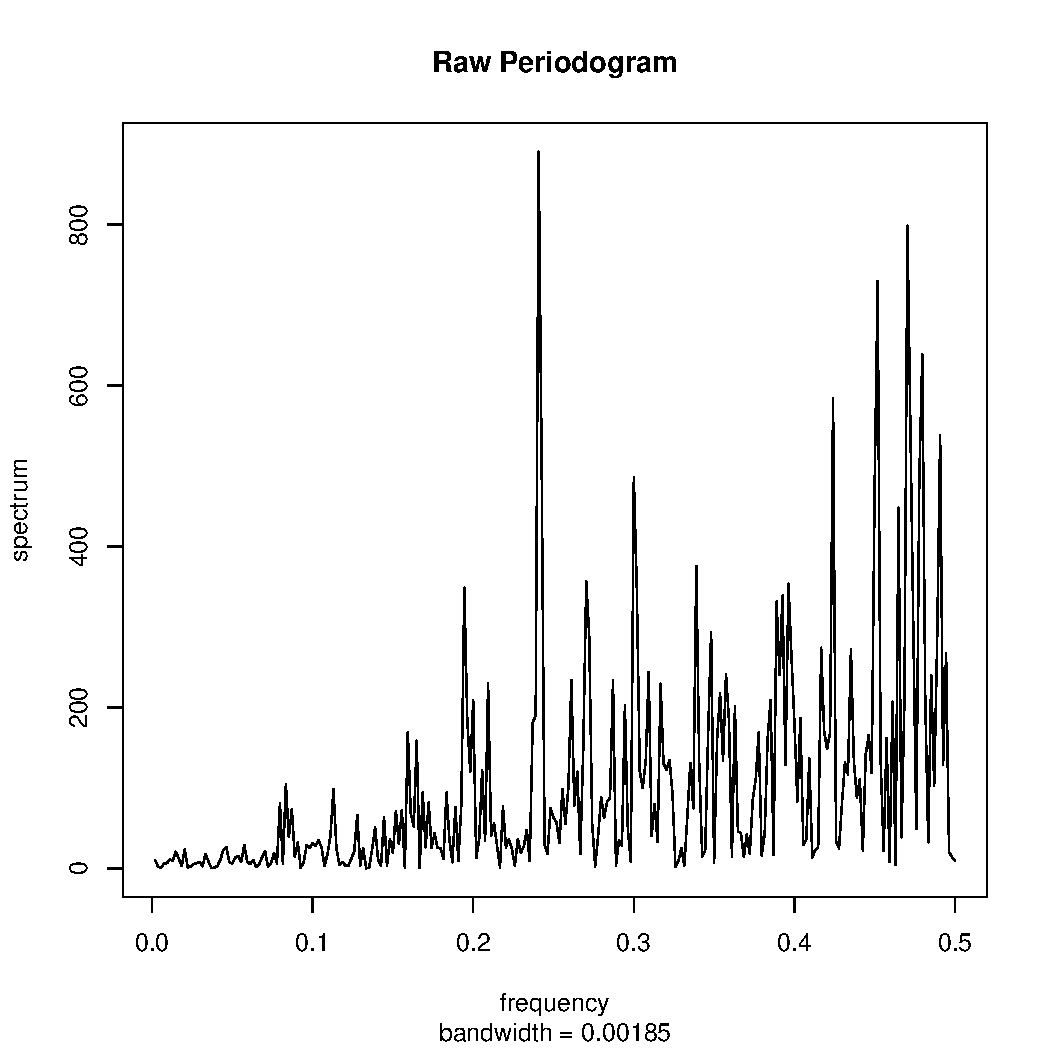
\includegraphics[width=0.45\linewidth]{../image/raw_periodogram.pdf}
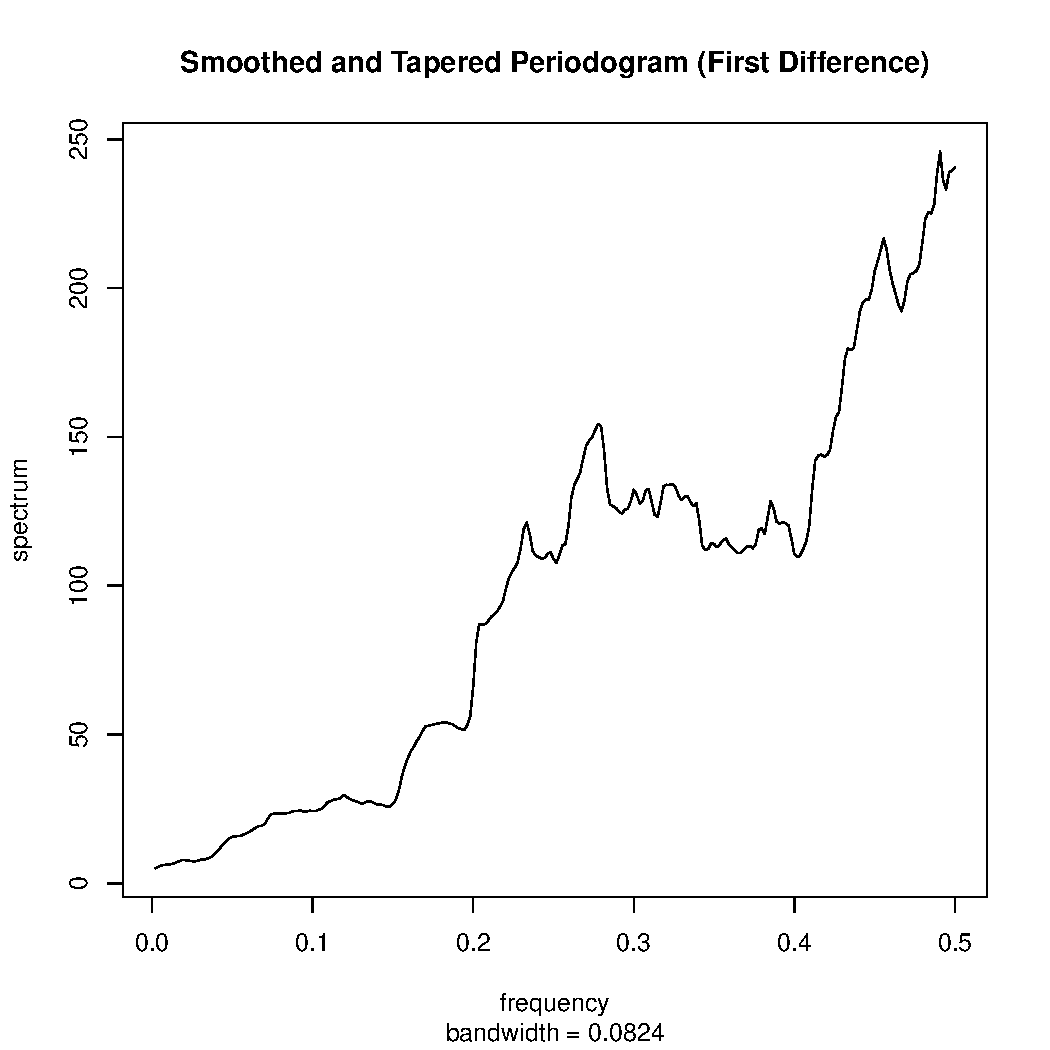
\includegraphics[width=0.45\linewidth]{../image/smooth_tapered_periodogram.pdf}
\caption{The Periodogram (left) and a Smoothed and Tapered Periodogram (right). Smoothed with a Daniell Kerenel with window??TODO?? size $m = \sqrt{n} \approx 22$ and tapered with ??cosine bell taper with? ?val? $0.1$}
\label{periodogram}
\end{figure}



\begin{figure}
\centering
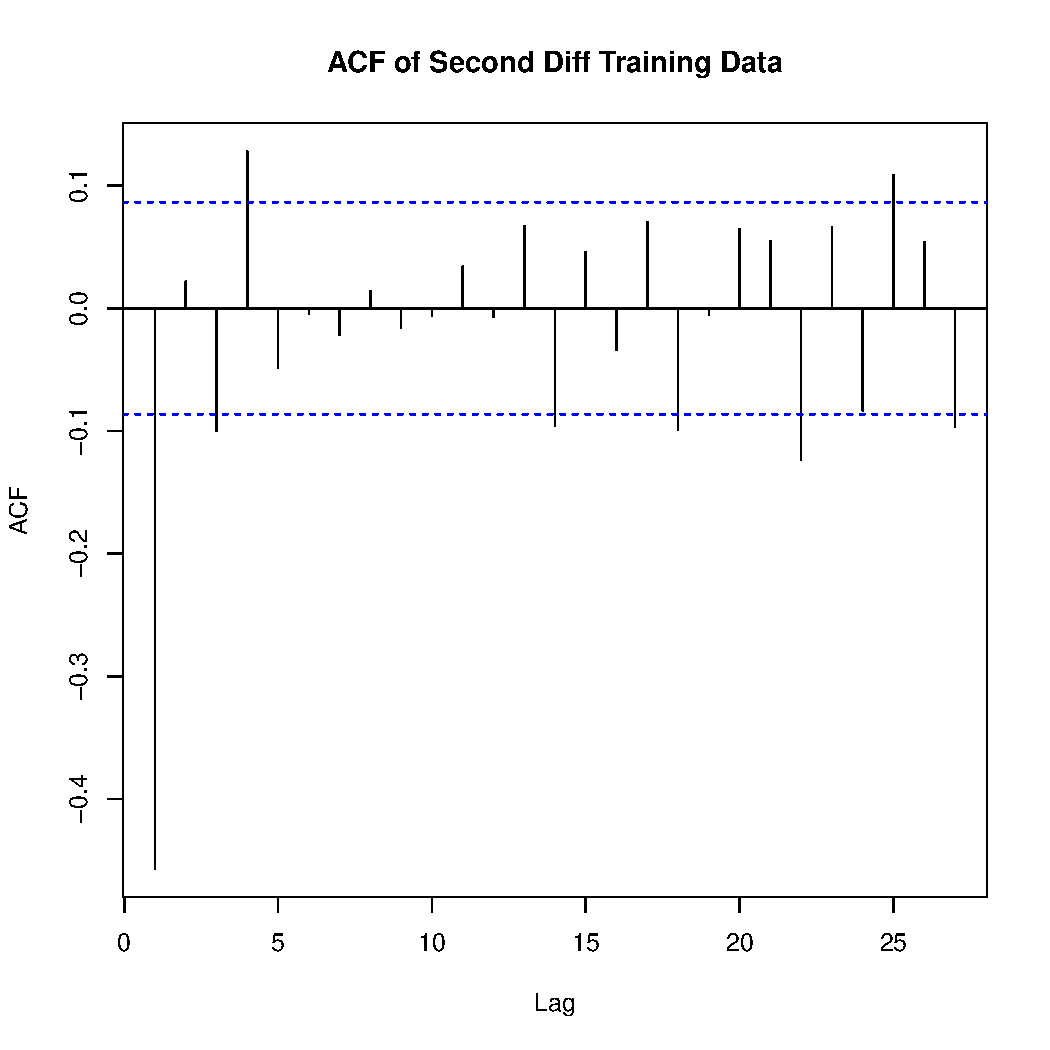
\includegraphics[width=0.45\linewidth]{../image/acf_second_diff.pdf}
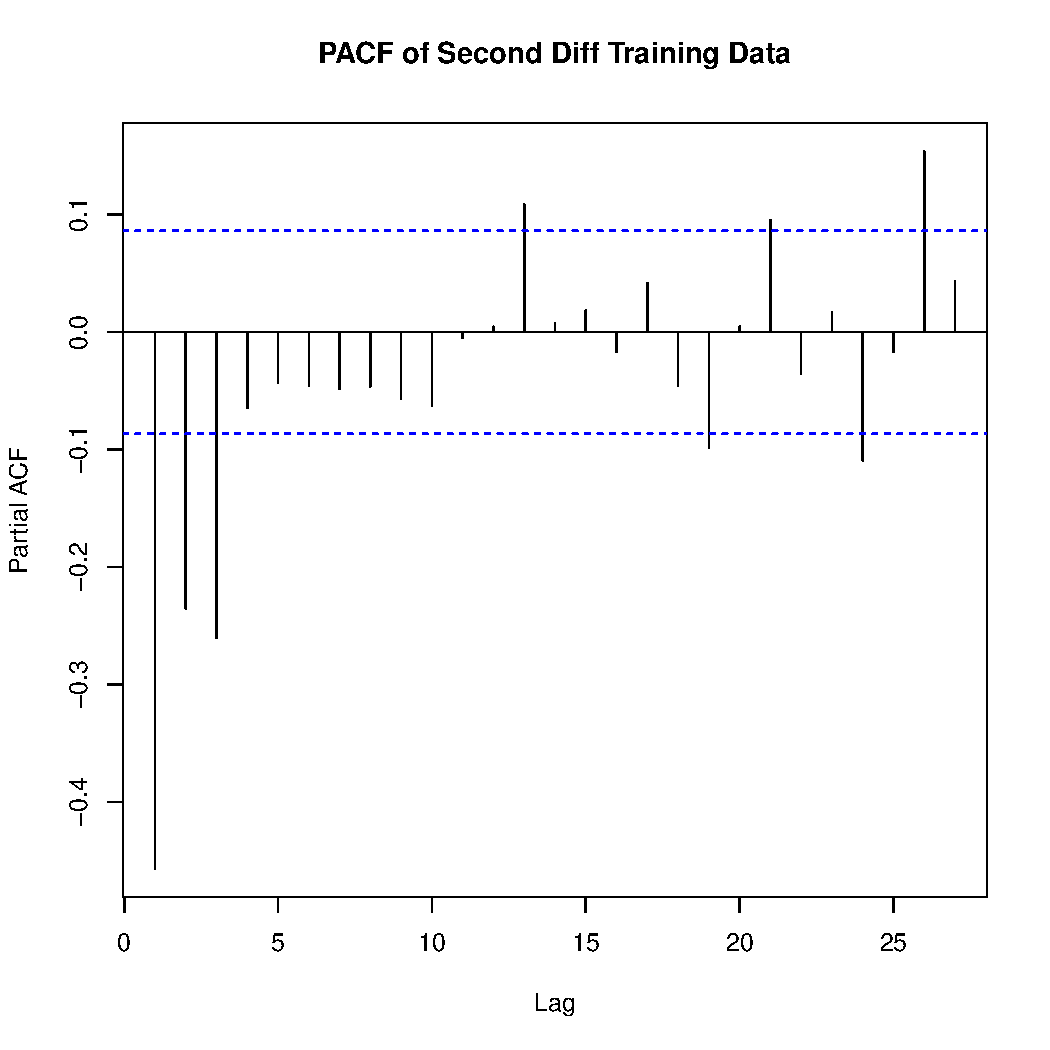
\includegraphics[width=0.45\linewidth]{../image/pacf_second_diff.pdf}
\caption{The ACF and PACF of the second diff time series}
\label{second_acf_pacf}
\end{figure}

\begin{figure}
\centering
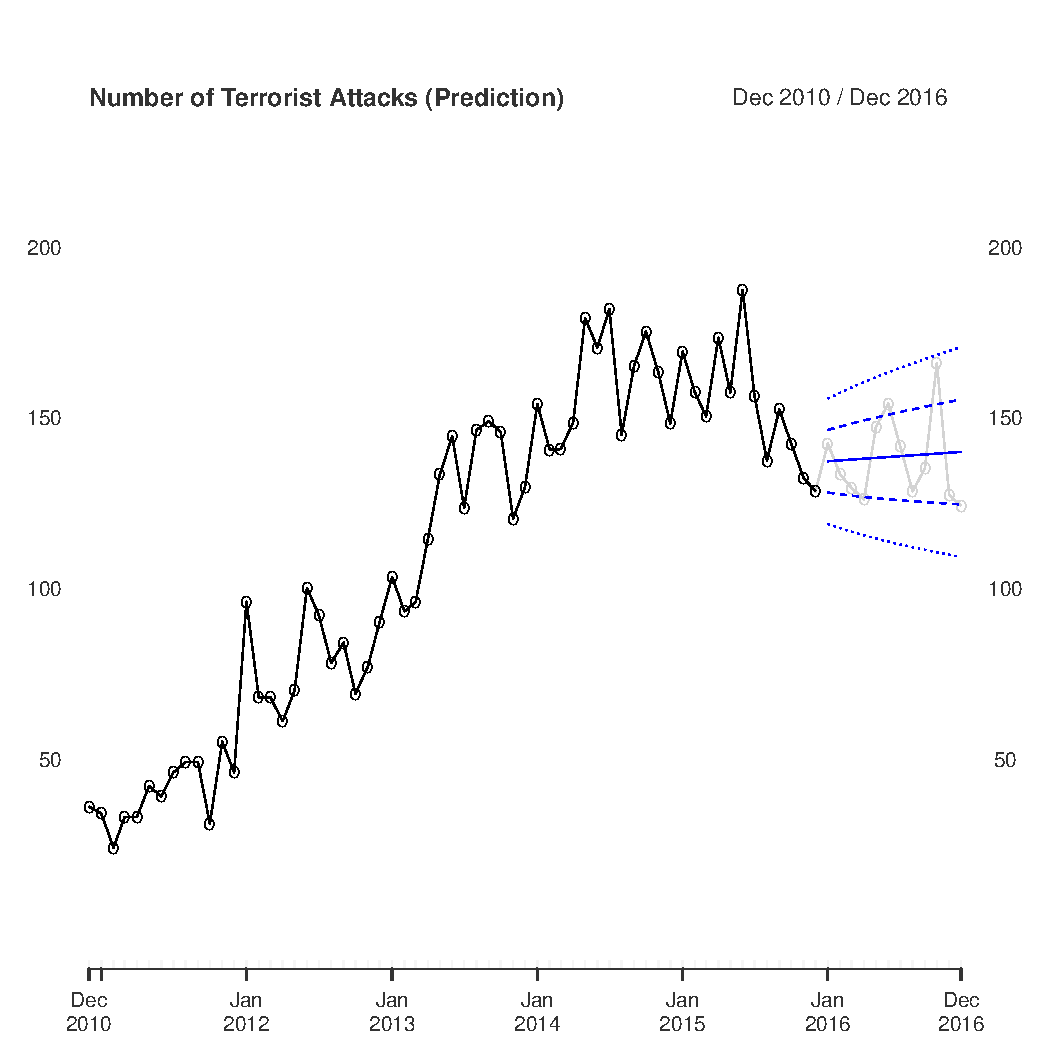
\includegraphics[width=0.75\linewidth]{../image/prediction_on_testing.pdf}
\caption{We use the model ---------- to generate a 12 month prediction denoted by the blue line. 1 sd and 2 sd error bars are the dotted lines. What actually occured is shown by the light gray.}
\label{prediction}
\end{figure}

\begin{figure}[t]
\centering
    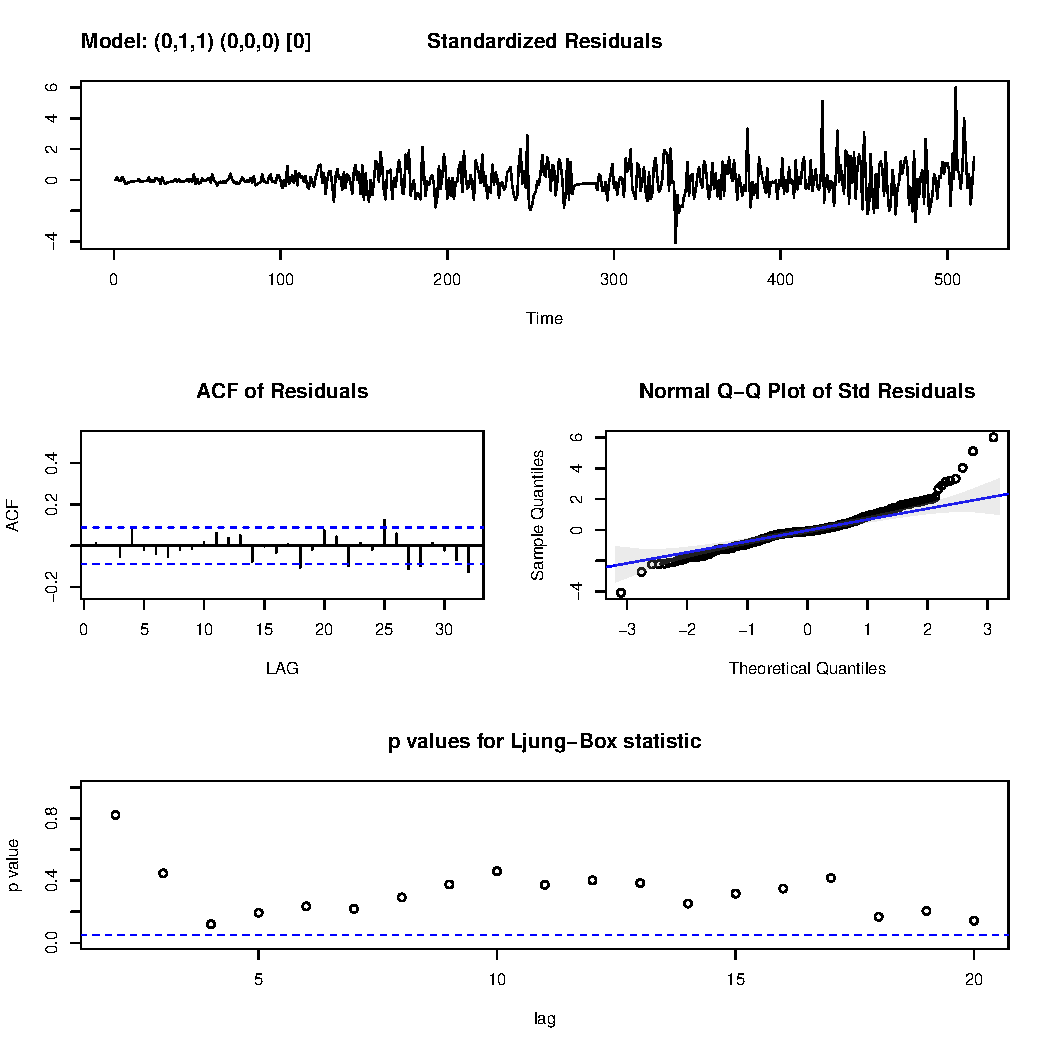
\includegraphics[width=0.75\textwidth]{../image/best_model.pdf}
\caption{This is the information from our best model.}
\label{outlier}
\end{figure}


\section{Methodology}
\section{Results}
\section{Discussion}
\section{Conclusion}

From the 
\begin{table}
\centering
\begin{tabular}{r || r | r| r| r}
$(p, d, q) \times(P, D, Q)_s$   & AIC   &AICc   &BIC    &MSE\\
\hline
$(0, 1, 1)$               & 5.248 &5.252  &4.265  &14907\\
$(0, 1, 1) \times (1, 0, 1)_4$   & 5.237 &5.241  &4.270  &14578.57\\ % Small p-values and passes ljung box p-values on seasonal ar1 and ma1; passes ljung box
$(0, 1, 1) \times (1, 1, 1)_4$   & 5.249 &5.254  &4.274  &14183.01\\
$(0, 1, 1) \times (1, 1, 2)_4$   & 5.242 &5.246  &4.275  &14934.03\\
\hline
$(1, 1, 2)$               & 5.256 & 5.260 &4.288  &15044.47\\
$(1, 1, 2) \times (1, 0, 1)_4$   & 5.243 &5.247  &4.292  &15130.19\\ %Large p-values on ma2, small 
$(1, 1, 2) \times (1, 1, 1)_4$   & 5.252 & 5.257 &4.294  &15197.85\\
$(1, 1, 2)\times (1, 1, 2)_4$   & 5.250 & 5.254 & 4.299 &15074.55
\end{tabular}
\caption{The metrics associated with different SARIMA models denoted by the left hand column.}
\end{table}

%For (terror4, 0, 1, 4, 1, 0, 1, 4) only ma1 coefficient was significant; it did pass ljung box.

\begin{table}
\centering
\begin{tabular}{r || r | r| r| r | r | r| r| r}%| r| r | r| r| r| r}
 AR/MA &0& 1& 2& 3& 4& 5& 6& 7\\%& 8& 9& 10& 11& 12& 13 \\
 \hline
 \hline
0&x&o&x&x&o&o&o&o\\%&o&o&o&o&o&x\\
1&x&x&o&x&o&o&o&o\\%&o&o&o&o&o&o\\
2&x&x&x&x&o&o&o&o\\%&o&o&o&o&o&o\\
3&x&x&x&x&o&o&o&o\\%&o&o&o&o&o&o\\
4&x&o&o&o&o&o&o&o\\%&o&o&o&o&o&o\\
5&x&x&o&o&o&o&o&o\\%&o&o&o&o&o&o\\
6&x&x&o&o&o&o&o&o\\%&o&o&o&o&o&o\\
7&x&x&o&o&o&o&o&o\\%&o&o&o&o&o&o
\end{tabular}
\begin{tabular}{r || r | r| r| r | r | r| r| r}%| r| r | r| r| r| r}
AR/MA&  0 &1& 2 &3& 4& 5& 6& 7\\%& 8& 9& 10& 11 &12 &13\\
\hline
\hline
0&x&x&x&x&o&o&o&o\\%&o&o&o&o&o&x\\
1&x&x&x&x&o&o&o&o\\%&o&o&o&o&o&o\\
2&x&x&x&x&o&o&o&o\\%&o&o&o&o&o&o\\
3&x&o&o&o&o&o&o&o\\%&o&o&o&o&o&o\\
4&x&x&o&o&o&o&o&o\\%&o&o&o&o&o&o\\
5&x&x&o&o&o&o&x&o\\%&o&o&o&o&o&o\\
6&x&x&x&o&o&o&o&o\\%&o&o&o&o&o&o\\
7&x&x&o&o&o&o&o&o\\%&o&o&o&o&o&o
\end{tabular}
\caption{The EACF table for once diffed (left) and twice diffed data (right).}
\end{table}





\end{document} 

